\chapter{Data acquisition for CHIPS} %%%%%%%%%%%%%%%%%%%%%%%%%%%%%%%%%%%%%%%%%%%%%%%%%%%%%%%%%%%%%
\label{chap:daq} %%%%%%%%%%%%%%%%%%%%%%%%%%%%%%%%%%%%%%%%%%%%%%%%%%%%%%%%%%%%%%%%%%%%%%%%%%%%%%%%%

The primary task of any Data Acquisition system is the processing of low-level signals measuring
real-world physics and their transfer to permanent storage for further analysis. Commonly, this
procedure also includes decision making as to whether the signal is deemed interesting enough to
record, known as a \emph{trigger}. Both these tasks can make DAQ systems incredibly complex,
especially when they must operate in an efficient and resilient manner for vast amounts of data in
real-time, while also providing detector control and monitoring.

In the context of the \chips project, the DAQ system records all PMT hits, timestamps them using a
common clock, and transfers them out of the detector to a central processing node. This node then
applies a trigger to select hits that fall within the interesting \numi beam spill time window,
before the selected hits are sliced into events and moved to permanent storage for further
analysis. Alongside these processes, the DAQ system also configures the detector and provides data
quality and detector component monitoring.

Although relatively simple when compared to the incredibly complex and time-pressured DAQ systems
of the LHC experiments, the DAQ system developed for the \chips project introduces some novel
approaches to solve the unique constraints of the \chips concept. Namely, deployment within a body
of water and a limited resource budget. In this chapter, the DAQ system for \chips as applied to
the \chipsfive prototype detector module is described alongside highlighting any novel approaches.
The description is presented in two broad categories, hardware and software, with a short
description of the timing system beforehand.

\section{White Rabbit timing} %%%%%%%%%%%%%%%%%%%%%%%%%%%%%%%%%%%%%%%%%%%%%%%%%%%%%%%%%%%%%%%%%%%%
\label{sec:daq_timing} %%%%%%%%%%%%%%%%%%%%%%%%%%%%%%%%%%%%%%%%%%%%%%%%%%%%%%%%%%%%%%%%%%%%%%%%%%%

To ensure PMT hit times are synchronised throughout \chips detectors, a common clock must be
shared across all timestamping electronics. For this purpose, \chips uses a \emph{White Rabbit}
(WR) network~\cite{lipinski2011}. Initially developed at CERN, the open-source WR project provides
an ethernet-based time distribution network with sub-nanosecond synchronisation accuracy between
nodes. By using two-way exchanges of WR messages, precise adjustment of individual node clock
phases and offsets is possible across thousands of devices, separated by tens of kilometres. All
of this is achieved in parallel with a standard data transfer network capable of
\unit{1}{\text{Gb}} speeds.

All nodes are synchronised to the clock of a \emph{GrandMaster} node, typically a WR
\emph{switch}, the most common WR hardware component. As input, the switch receives an IRIG-B
(Inter-Range Instrumentation Group timecode B) and a \unit{10}{\text{MHz}} signal from a GPS
disciplined oscillator. These inputs allow for synchronisation of the GrandMaster clock to
International Atomic Time (TAI). As \chips detector modules require synchronisation to accelerator
clocks many hundreds of kilometres away to determine the arrival time of beam spills, the GPS
disciplined timing is particularly important.

WR hardware is commercially available from many vendors. Within \chipsfive, two WR devices are
used for time synchronisation and data transfer, both shown in Fig.~\ref{fig:wr_electronics}.
Firstly, a compact version of the standard WR switch~\cite{wrswitch2020}, specially developed for
the \chips project at Nikhef~\cite{wrchromium2020}. Secondly, a WR-LEN (Lite Embedded Node) from
Seven Solutions~\cite{wrlen2020}. 

\begin{figure} % WHITE-RABBIT COMPONENTS DIAGRAM %
    \centering
    \subcaptionbox{White Rabbit switch}{%
        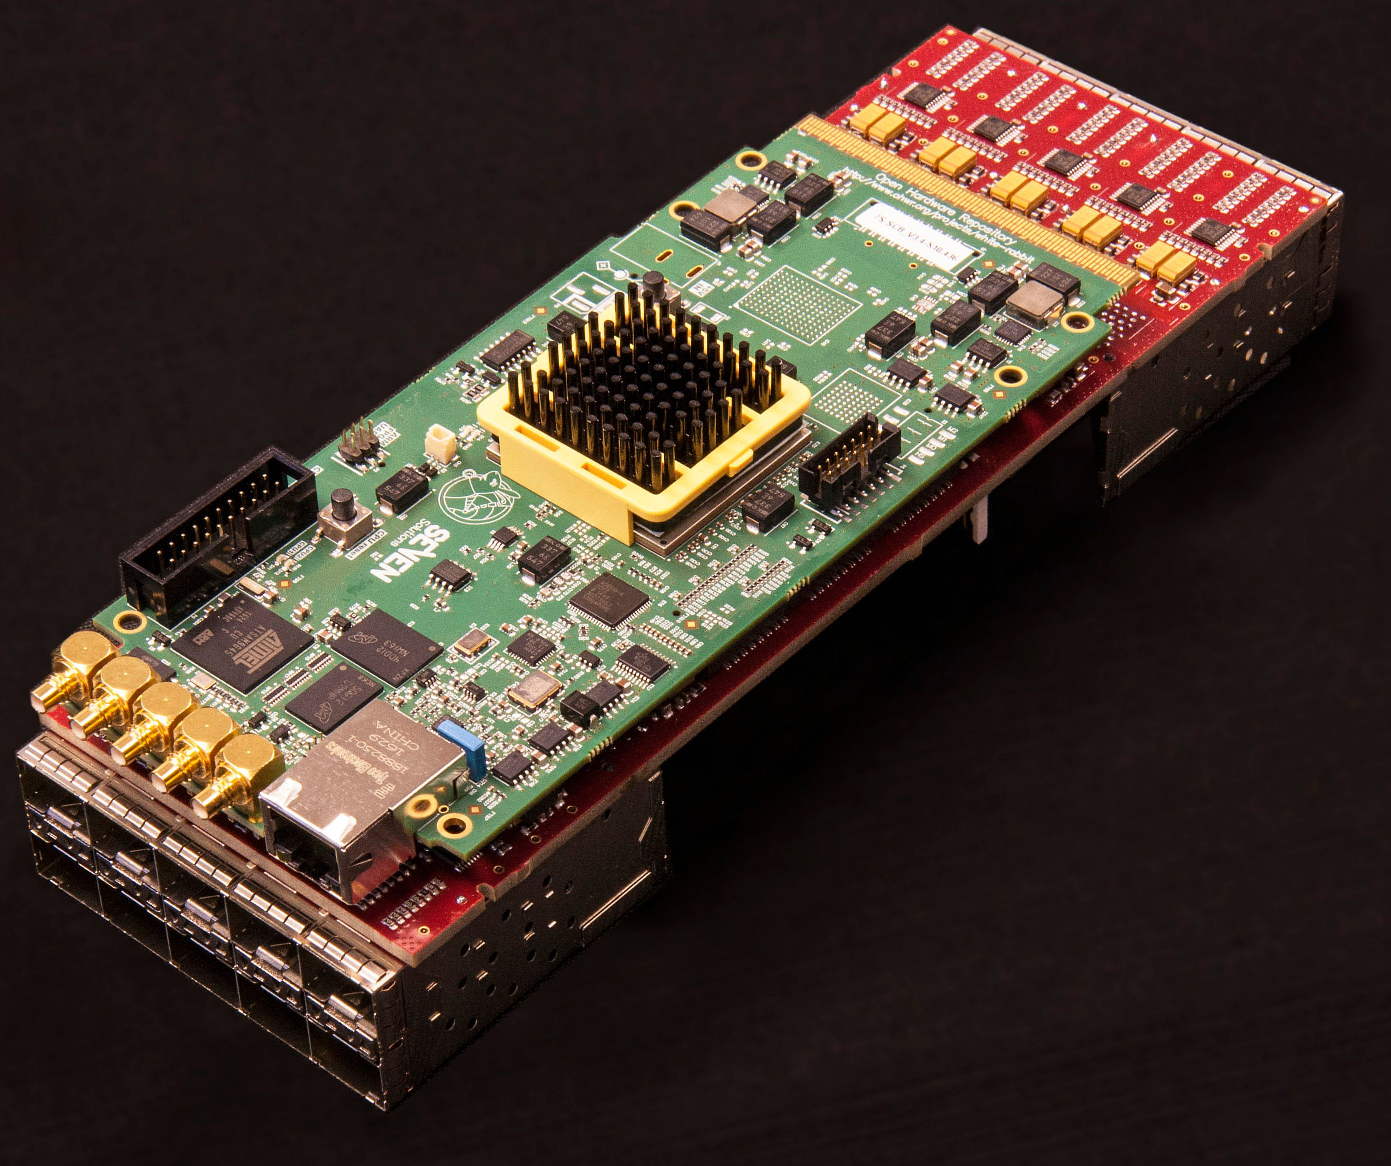
\includegraphics[height=6cm]{diagrams/5-daq/wr_switch.pdf}%
    }
    \quad
    \subcaptionbox{White Rabbit LEN}{%
        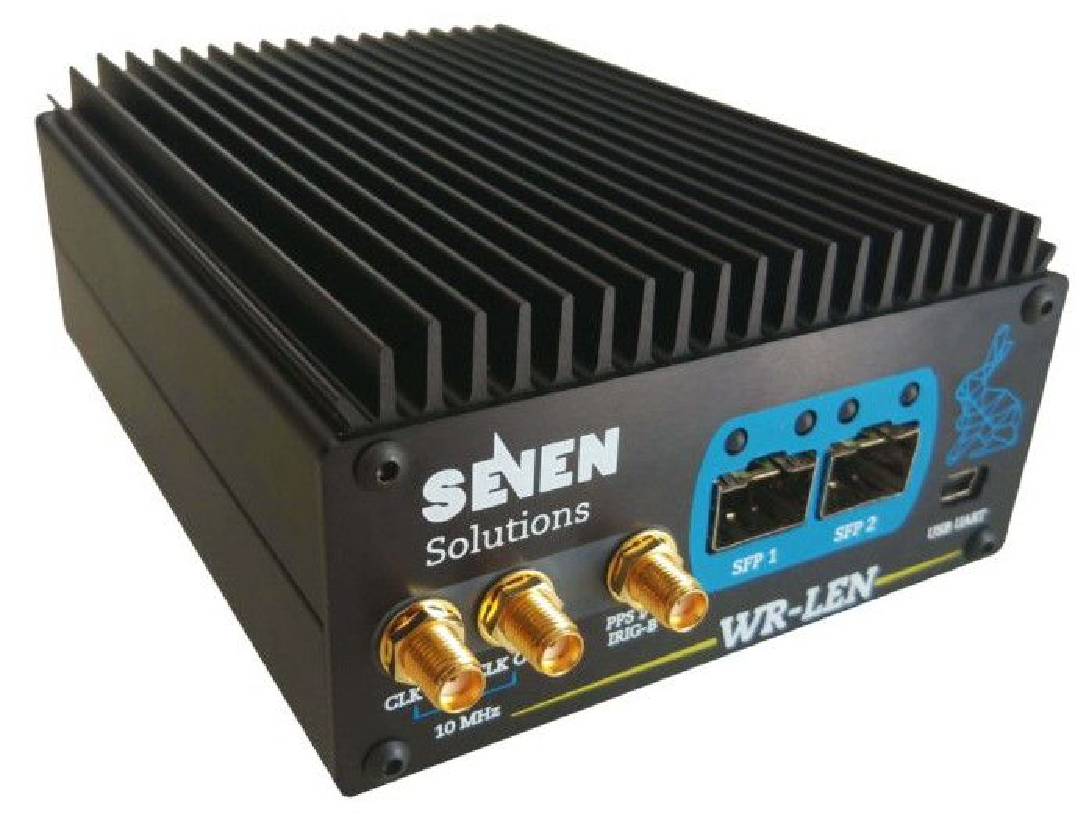
\includegraphics[height=6cm]{diagrams/5-daq/wr_len.pdf}%
    }
    \caption[Pictures of the White Rabbit timing hardware used within \chipsfive]
    {Pictures of the White Rabbit timing hardware used within \chipsfive. The compact White rabbit
        switch  specially designed for \chips is shown in (a), while the White Rabbit Lite
        Embedded Node (WR-LEN) from Seven Solutions is shown in (b).}
    \label{fig:wr_electronics}
\end{figure}

All WR components are connected using \unit{1}{\text{Gb}} bi-directional optical fibre
connections, using the \unit{1310}{\text{nm}} and \unit{1550}{\text{nm}} wavelengths via Small
Form-Factor Pluggable Transceivers (SFPs). Fig.~\ref{fig:sync} shows the subsequent WR
synchronised pulse per second clock rising edges for two \chipsfive WR switches separated by
\unit{500}{\text{m}} of fibre. With the vertical ticks representing single nanoseconds,
sub-nanosecond time synchronisation accuracy between the switches is observed.

\begin{figure} % WHITE-RABBIT SYNC DIAGRAM %
    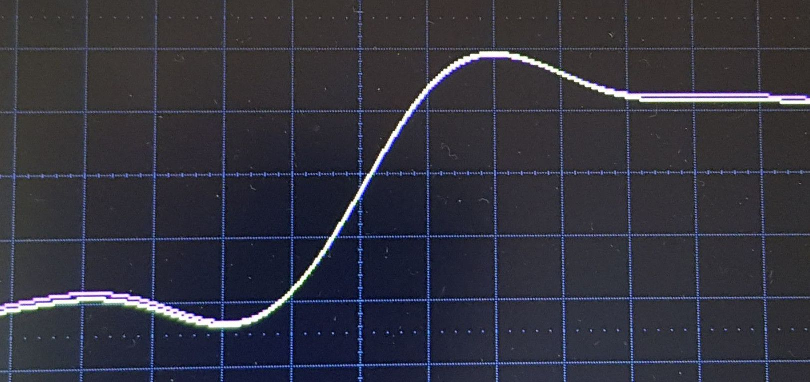
\includegraphics[width=0.7\textwidth]{diagrams/5-daq/sync.pdf}
    \caption[Picture of White Rabbit timing synchronisation seen within \chipsfive]
    {Picture of an oscilloscope display measuring the pulse per second output signal from two WR
        switches shown in pink and yellow at either end of a \unit{500}{\text{m}} long optical
        fibre. The vertical ticks are in nanoseconds showing the sub-nanosecond synchronisation
        possible with the WR timing network.}
    \label{fig:sync}
\end{figure}

\section{Hardware} %%%%%%%%%%%%%%%%%%%%%%%%%%%%%%%%%%%%%%%%%%%%%%%%%%%%%%%%%%%%%%%%%%%%%%%%%%%%%%%
\label{sec:daq_hard} %%%%%%%%%%%%%%%%%%%%%%%%%%%%%%%%%%%%%%%%%%%%%%%%%%%%%%%%%%%%%%%%%%%%%%%%%%%%%

The hardware of the \chipsfive DAQ system is split into two distinct implementations at its lower
levels (closest to the PMTs), corresponding to the Nikhef and Madison \textsc{Pom} types. \chips
R\&D efforts have principally developed the novel Madison implementation with the view to use this
hardware within detector modules exclusively. However, as a safe stepping stone, while development
and testing are still ongoing, \chipsfive mainly contains proven Nikhef hardware developed for the
KM3NeT experiment~\cite{adrian2016}.

The complete DAQ and power distribution system for \chipsfive is diagrammatically shown in
Fig.~\ref{fig:daq}. The following subsections describe each component, starting from the lowest
level and working upwards. The Nikhef and Madison descriptions are separated for clarity as well
as the high-level combined hardware systems, part of which is not physically located within the
detector but onshore in an electronics hut (separate from the water filtration hut).

\begin{figure} % DAQ DIAGRAM %
    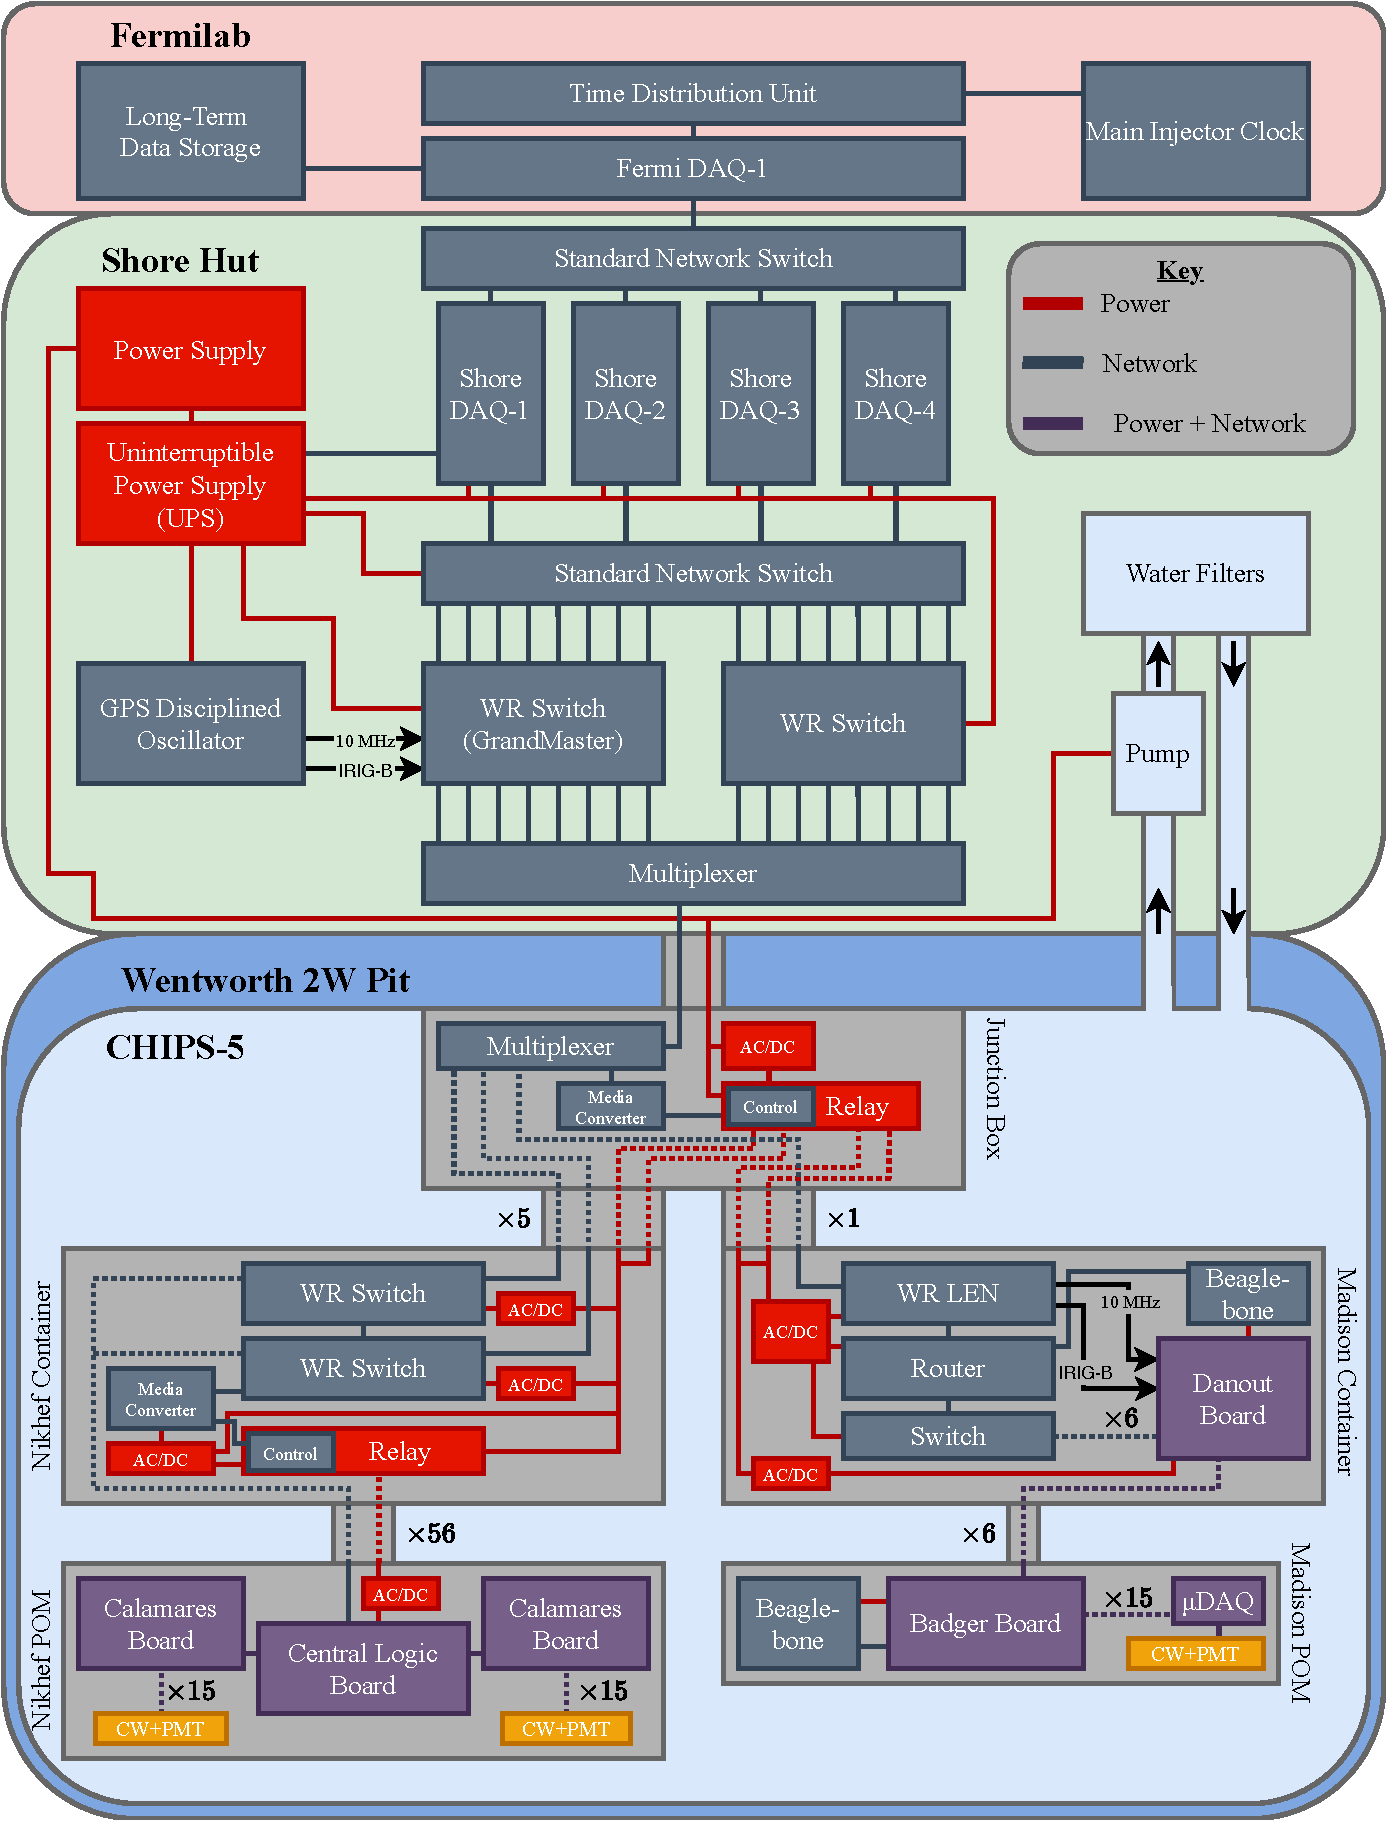
\includegraphics[width=\textwidth]{diagrams/5-daq/daq.pdf}
    \caption[Diagram of the complete \chipsfive data acquisition and power distribution system]
    {Diagram of the complete \chipsfive DAQ and power distribution system.}
    \label{fig:daq}
\end{figure}

Common to both low-level hardware implementations is the use of the Time over Threshold (ToT)
method for PMT signal digitisation. Each analogue PMT pulse is fed to a ToT discriminator coupled
with a Time to Digital Converter (TDC) to generate each digitised recorded hit, as shown in
Fig.~\ref{fig:tot}. Compared to the more common Analogue to Digital Converter (ADC) readout, ToT
values are less accurate and do not scale linearly with deposited charge. However, the ToT
methodology is used within \chips as the electronics is simpler and notably cheaper.

\begin{figure} % TOT DIAGRAM DIAGRAM %
    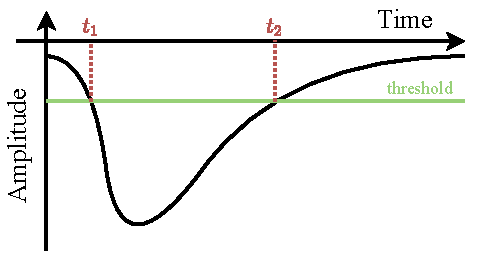
\includegraphics[width=0.6\textwidth]{diagrams/5-daq/tot.pdf}
    \caption[Illustrative diagram showing how Time over Threshold is measured]
    {Illustrative diagram showing how a ToT value is measured. As soon as the rising edge of a PMT
        charge pulse rises above a given threshold (goes below in the negative charge case) a time
        is recorded $t_{1}$, when the falling edge later falls below the threshold a second time
        $t_{2}$ is recorded. The difference in time between $t_{1}$ and $t_{2}$ is output by the
        electronics as a digitised ToT value.}
    \label{fig:tot}
\end{figure}

\subsection{Nikhef hardware} %%%%%%%%%%%%%%%%%%%%%%%%%%%%%%%%%%%%%%%%%%%%%%%%%%%%%%%%%%%%%%%%%%%%%
\label{sec:daq_hard_Nikhed} %%%%%%%%%%%%%%%%%%%%%%%%%%%%%%%%%%%%%%%%%%%%%%%%%%%%%%%%%%%%%%%%%%%%%%

All Nikhef HZC PMTs are attached directly to a simple readout board containing a high-voltage
generating Cockcroft-Walton circuit. Up to 30 such PMTs are connected to two \emph{Calamares}
boards within the electronics box of each Nikhef \textsc{Pom} via standard category 5 cables with
RJ45 connectors, as shown in Fig.~\ref{fig:nikhef_plane}. Both Calamares boards are directly
attached to a \emph{Central Logic Board} (CLB)~\cite{biagi2015, eijk2015}. The CLB contains ToT
discriminators and TDCs to digitise the recorded signals as well as electronics to synchronise to
the WR network clock for timestamping. Each Nikhef \textsc{Pom} electronics box also contains an
AC to DC power converter (AC/DC) whose output is fed into the CLB for power distribution.

\begin{figure} % NIKHEF PLANE DIAGRAM %
    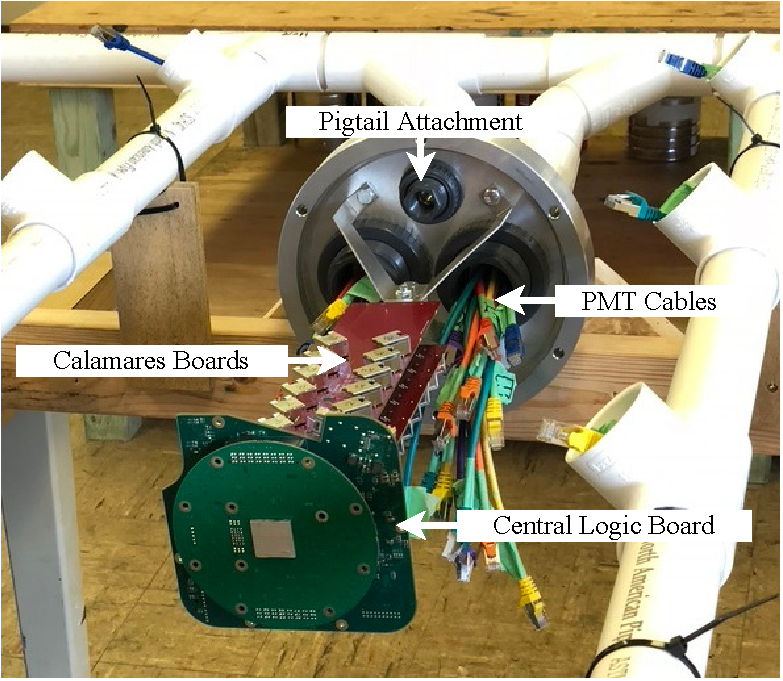
\includegraphics[width=0.8\textwidth]{diagrams/5-daq/nikhef_plane.pdf}
    \caption[Labelled picture of the Nikhef \textsc{Pom} electronics box]
    {Labelled picture of the Nikhef \textsc{Pom} electronics box without its aluminium casing.
        Both ends of the category 5 PMT cables can be seen, either at the PMT mounting points or
        entering the electronics box and not yet plugged into Calamares boards.}
    \label{fig:nikhef_plane}
\end{figure}

Every Nikhef \textsc{Pom} is connected via a single optical fibre and a single power connection to
a \emph{Nikhef-container}, the contents of which are labelled in the bottom half of
Fig.~\ref{fig:full_setup}. Two WR switches are used within each container to provide sufficient
\textsc{Pom} networking ports. Both switches are powered by independent AC to DC converters and
connected via a single optical fibre each to the higher level DAQ systems. An additional
connection between each switch ensures that if one higher-level connection fails the other can
still be used.

Each Nikhef-container also contains a relay board to control the power supply to individual
\textsc{Pom}s. The relay board control electronics are powered via an AC to DC converter and
connected to one of the switches via a media converter for networking. The media converter is
required to convert the optical fibre WR switch connection to a standard RJ45 copper cable
connection. A total of five Nikhef-containers are present within \chipsfive.

\begin{figure} % FULL SETUP DIAGRAM %
    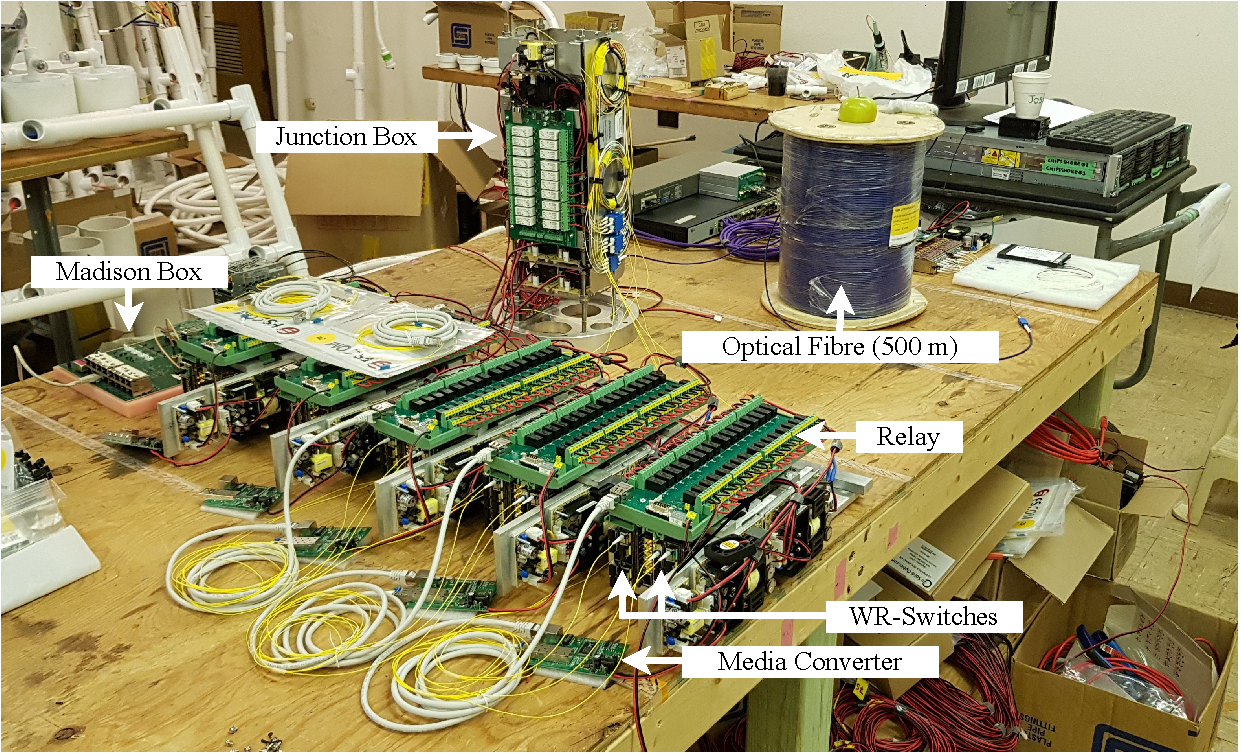
\includegraphics[width=\textwidth]{diagrams/5-daq/full_setup.pdf}
    \caption[Picture of the non \textsc{Pom} components of the \chipsfive DAQ system]
    {Picture of the non \textsc{Pom} components of the \chipsfive DAQ system arranged on a table
        at the PolyMet mining administration building.}
    \label{fig:full_setup}
\end{figure}

\subsection{Madison hardware} %%%%%%%%%%%%%%%%%%%%%%%%%%%%%%%%%%%%%%%%%%%%%%%%%%%%%%%%%%%%%%%%%%%%
\label{sec:daq_hard_madison} %%%%%%%%%%%%%%%%%%%%%%%%%%%%%%%%%%%%%%%%%%%%%%%%%%%%%%%%%%%%%%%%%%%%%

Every Madison Hamamatsu PMT is directly attached to a high-voltage generating Cockcroft-Walton
board followed by a signal processing $\micro$DAQ, as shown in
Fig.~\ref{fig:madison_pmt_assembly}. The $\micro$DAQ is a small microcontroller developed for both
IceCube and \chips at WIPAC in Madison. Capable of timestamping and digitising signals directly at
the PMT level, the $\micro$DAQ also sets the PMT operating voltage by controlling the driving
frequency of the Cockcroft-Walton board~\cite{eijk2018}.

Up to 16 $\micro$DAQs receive power, networking, and WR synchronised IRIG-B and
\unit{10}{\text{MHz}} timing signals from a \emph{badger-board}, as shown in
Fig.~\ref{fig:madison_plane}. Standard category 5 cables with RJ45 connectors are used for these
connections. The badger-board is located within the electronics box of each Madison \textsc{Pom}
and acts as a simple fanout and power control board. For logic, each badger-board has an attached
mezzanine Beaglebone~\cite{beagle2020}. This single-board Linux machine (very similar to a
Raspberry Pi) controls the power supply to, and receives hits from, the attached $\micro$DAQs.

\begin{figure} % MADISON PLANE DIAGRAM %
    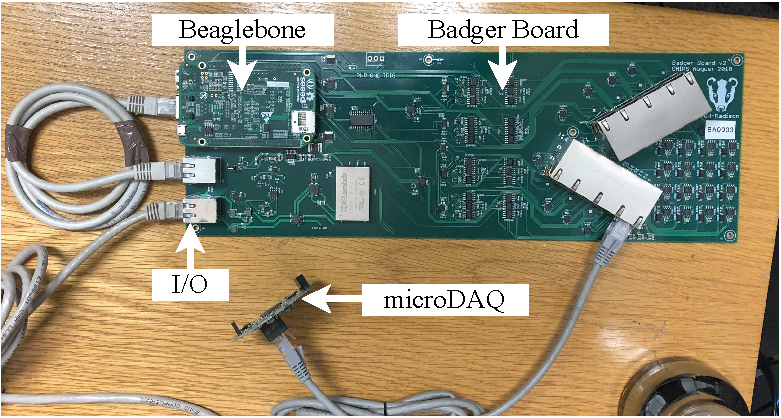
\includegraphics[width=0.8\textwidth]{diagrams/5-daq/madison_plane.pdf}
    \caption[Labelled picture of the components of the Madison \textsc{Pom} electronics box]
    {Labelled picture of the components of the Madison \textsc{Pom} electronics box.}
    \label{fig:madison_plane}
\end{figure}

Similarly, up to 16 Madison \textsc{Pom} badger-boards receive power, networking and WR
synchronised IRIG-B and \unit{10}{\text{MHz}} timing signals from a \emph{danout-board} located
within a single \emph{Madison-container}. Again, standard category 5 cables with RJ45 connectors
are used for these connections. The full contents of the Madison-container are shown in
Fig.~\ref{fig:madison_box}. Similar to the badger-board, the danout-board acts as a simple fanout
and power control board with an attached mezzanine Beaglebone. However, in this case, the attached
Beaglebone acts only to control the power provided by the danout-board.

PMT hits and other packets are instead routed through the danout-board into a networking stack.
Consisting of a WR-LEN, a router (required due to the limited WR-LEN routing table size), and a
switch (non WR), the stack provides networking to the higher-level DAQ via a single optical fibre.
The WR clock synchronised IRIG-B and \unit{10}{\text{MHz}} timing signals are output by the WR-LEN
to the danout-board for forwarding to the lower-level components. Additionally, two AC to DC
converters provide power for both the devices within the container and all lower-level components
via the danout-board.

\begin{figure} % MADISON BOX DIAGRAM %
    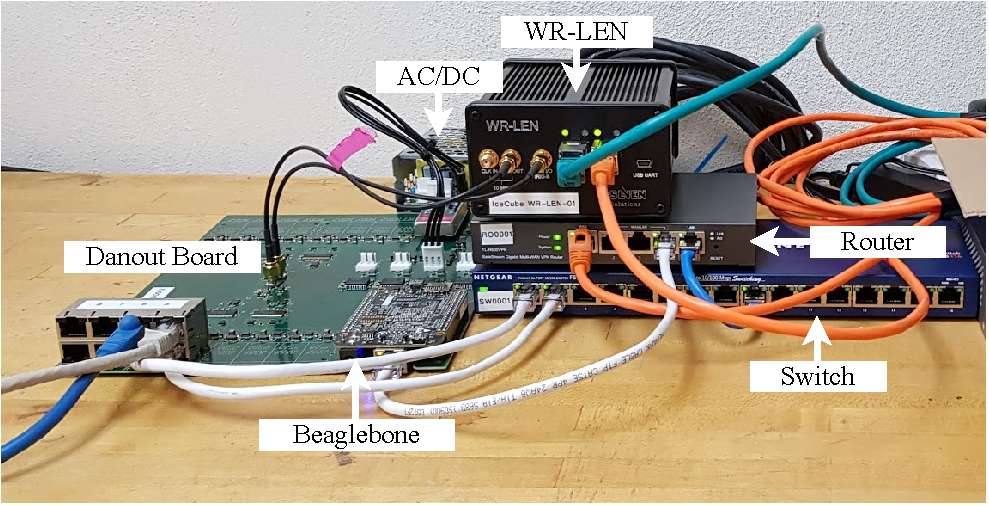
\includegraphics[width=\textwidth]{diagrams/5-daq/madison_box.pdf}
    \caption[Labelled picture of the Madison-container components]
    {Labelled picture of the Madison-container components. The blue and grey cables exiting the
        left hand side of the image go to individual Madison \textsc{Pom}s connecting to the I/O
        port shown in fig.~\ref{fig:madison_plane}. An optical fibre connection into the left SFP
        port of the WR-LEN is used in reality rather than the copper connection shown here.}
    \label{fig:madison_box}
\end{figure}

Compared to the Nikhef hardware the Madison.
\begin{itemize}
    \item By leveraging commercially available Beaglebones ($\sim£50$ each) for onboard logic and
    using vastly \textbf{cheaper} WR-LENs compared to WR switches, the Madison DAQ hardware
    implementation is drastically cheaper compared to the Nikhef (KM3NeT) approach for a minimal
    reduction in performance.
    \item By having a fully fledged Linux machine on each POM and easily reprogrammable
    $\micro$DAQ microcontrollers the DAQ software can be easily \textbf{configurable} and upgraded
    once deployed. Having so much cheap general purpose processing power close to the PMTs allows
    for most of the computation to happen at that level, additional logic can be added. Don't even
    know what we could implement yet using it. Advanced processing at lower level. 
\end{itemize}

\subsection{Combined systems} %%%%%%%%%%%%%%%%%%%%%%%%%%%%%%%%%%%%%%%%%%%%%%%%%%%%%%%%%%%%%%%%%%%%
\label{sec:daq_hard_combined} %%%%%%%%%%%%%%%%%%%%%%%%%%%%%%%%%%%%%%%%%%%%%%%%%%%%%%%%%%%%%%%%%%%%

Each Nikhef-container and Madison-container is connected to a single \emph{junction-box}, labelled
in Fig.~\ref{fig:full_setup}. This central container acts as the interface between the detector
electronics and the umbilical carrying data and power between the shore and the detector. All
connections to the junction-box (as well as those between \textsc{Pom}s and Nikhef and Madison
containers) are made within watertight, flexible PVC tubing called \emph{manifolds}. These tubes
span all corners of the \chipsfive detector, as shown in Fig.~\ref{fig:manifold}.

\begin{figure} % MANIFOLD DIAGRAM %
    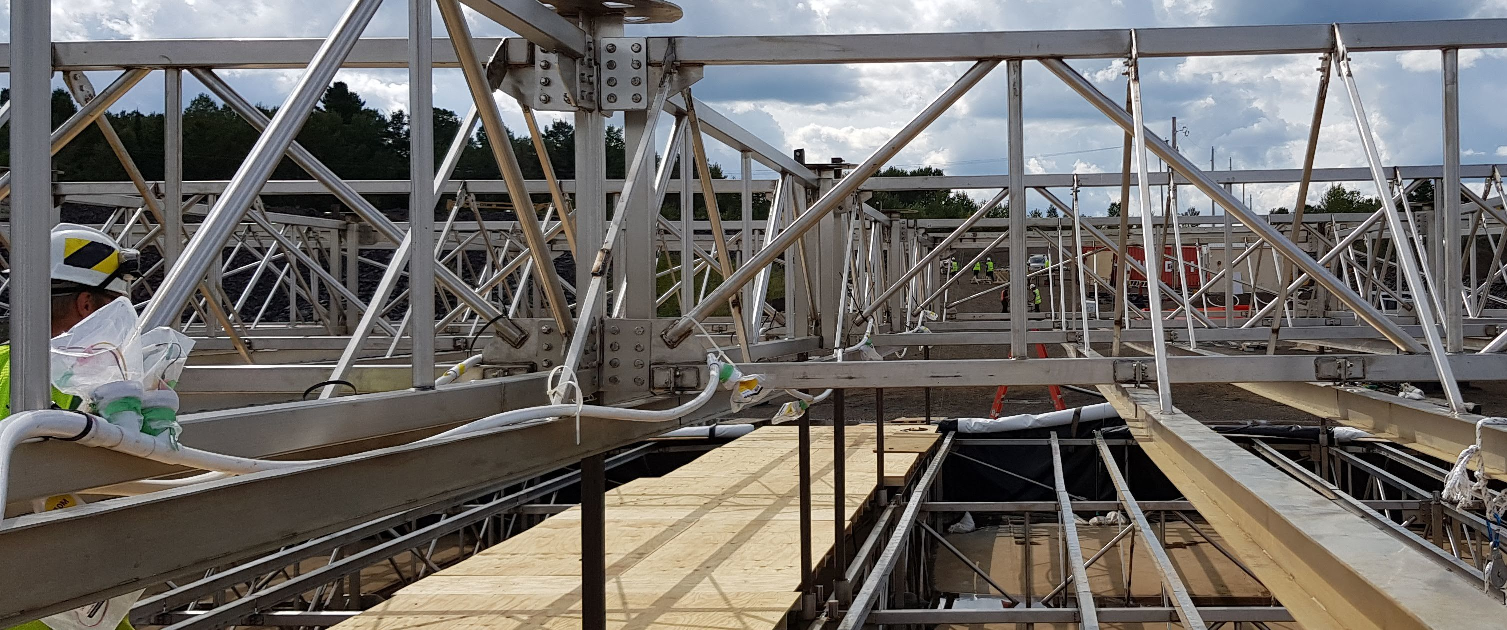
\includegraphics[width=\textwidth]{diagrams/5-daq/manifold.pdf}
    \caption[Picture of a manifold connection within the \chipsfive detector]
    {Picture of a Nikhef \textsc{Pom} to Nikhef-container manifold (in white) attached to the
        top-cap of the \chipsfive detector. In the left of the image, two unattached Nikhef
        \textsc{Pom} pigtail connections are seen, both covered in green tape and a plastic bag.}
    \label{fig:manifold}
\end{figure}

For networking the junction-box contains a Coarse Wavelength Division Multiplexing (CWDM)
multiplexer/demultiplexer (MUX/DEMUX). This device supports 32 wavelengths for a total of 16
bi-directional \unit{1}{\text{Gb}} connections over the single \unit{500}{\text{m}} long umbilical
optical fibre. Each WR-LEN or WR switch within the detector uses one of these channels exclusively
with the corresponding wavelength SFP.

The two umbilical power connections are distributed via two thick copper plates to all the relay
channels within the junction-box. Two relay boards are used to provide a sufficient number of
output channels, with their control electronics powered by separate AC to DC converters and each
connected to one of the multiplexer/demultiplexer networking channels via a media converter
(optical fibre to RJ45). Each relay channel also has a built-in \emph{trip gate} to immediately
power-off the channel if a current surge is detected. This protection is particularly crucial for
\chipsfive as water leaks are possible.

The contents of the DAQ electronics \emph{Shore Hut} are shown in Fig.~\ref{fig:hut_daq}. The
single umbilical optical fibre connection passes through a multiplexer/demultiplexer before each
of the wavelength-specific channels are passed into one of two WR switches. Multiple Virtual Local
Area Networks (VLANs) are configured on each switch such that for each wavelength channel only a
single paired port on the other physical side of the switch carries that channels data to and from
the standard networking switch (these connections are not present within Fig.~\ref{fig:hut_daq}).
Of the two WR switches, one is configured to be the GrandMaster with connections to a GPS
disciplined oscillator with an attached antenna. A single connection is also made between the WR
switches for clock synchronisation.

\begin{figure} % WHITE-RABBIT GM SETUP DIAGRAM %
    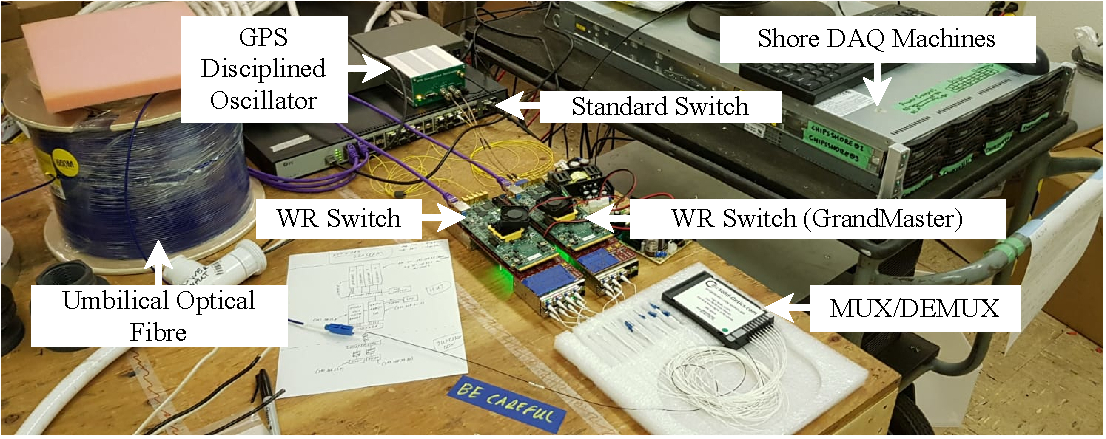
\includegraphics[width=\textwidth]{diagrams/5-daq/hut_daq.pdf}
    \caption[Picture of the onshore components of the \chipsfive DAQ system]
    {Picture of the onshore components of the \chipsfive DAQ system arranged on a table at the
        PolyMet mining administration building.}
    \label{fig:hut_daq}
\end{figure}

The standard network switch provides \unit{10}{\text{Gb}} connections to each of the Shore DAQ
computing machines whose specific roles are detailed in Section.~\ref{sec:daq_soft}. Each machine
is also connected to a second switch providing connections to the external internet and DAQ
components located at Fermilab. At Fermilab, a principle DAQ machine (Fermi DAQ-1) performs two
main roles. Firstly, it forwards \numi beam spill timing information from a Time Distribution Unit
attached to the Main Injector clock to \chipsfive. Secondly, it receives recorded detector data
from the \chipsfive located DAQ system and places it into long-term storage.

An uninterruptible power supply provides power to all devices within the Shore Hut, supplying
power for up to \unit{15}{\text{minutes}} after a power cut (sadly quite a common occurrence). The
two detector umbilical power connections do not use the uninterruptible supply and instead draw
power directly from the master supply, as does the water filtration pump.

\section{Software} %%%%%%%%%%%%%%%%%%%%%%%%%%%%%%%%%%%%%%%%%%%%%%%%%%%%%%%%%%%%%%%%%%%%%%%%%%%%%%%
\label{sec:daq_soft} %%%%%%%%%%%%%%%%%%%%%%%%%%%%%%%%%%%%%%%%%%%%%%%%%%%%%%%%%%%%%%%%%%%%%%%%%%%%%

The software of the \chipsfive DAQ system provides three main functionalities: control of the
detector instrumentation, the handling of recorded PMT hits, and the monitoring of hardware and
data quality. Each of these functions is discussed within a specific subsection below. Only the
high-level software components are detailed with the low-level CLB, Beaglebone, and $\micro$DAQ
software implementations omitted for brevity. An in-depth discussion of the CLB software can be
found in Ref.~\cite{aiello2019} while the Beaglebone and $\micro$DAQ software implementation can
be found at Ref.~\cite{microdaq2020}.

\begin{figure} % SOFTWARE DIAGRAM %
    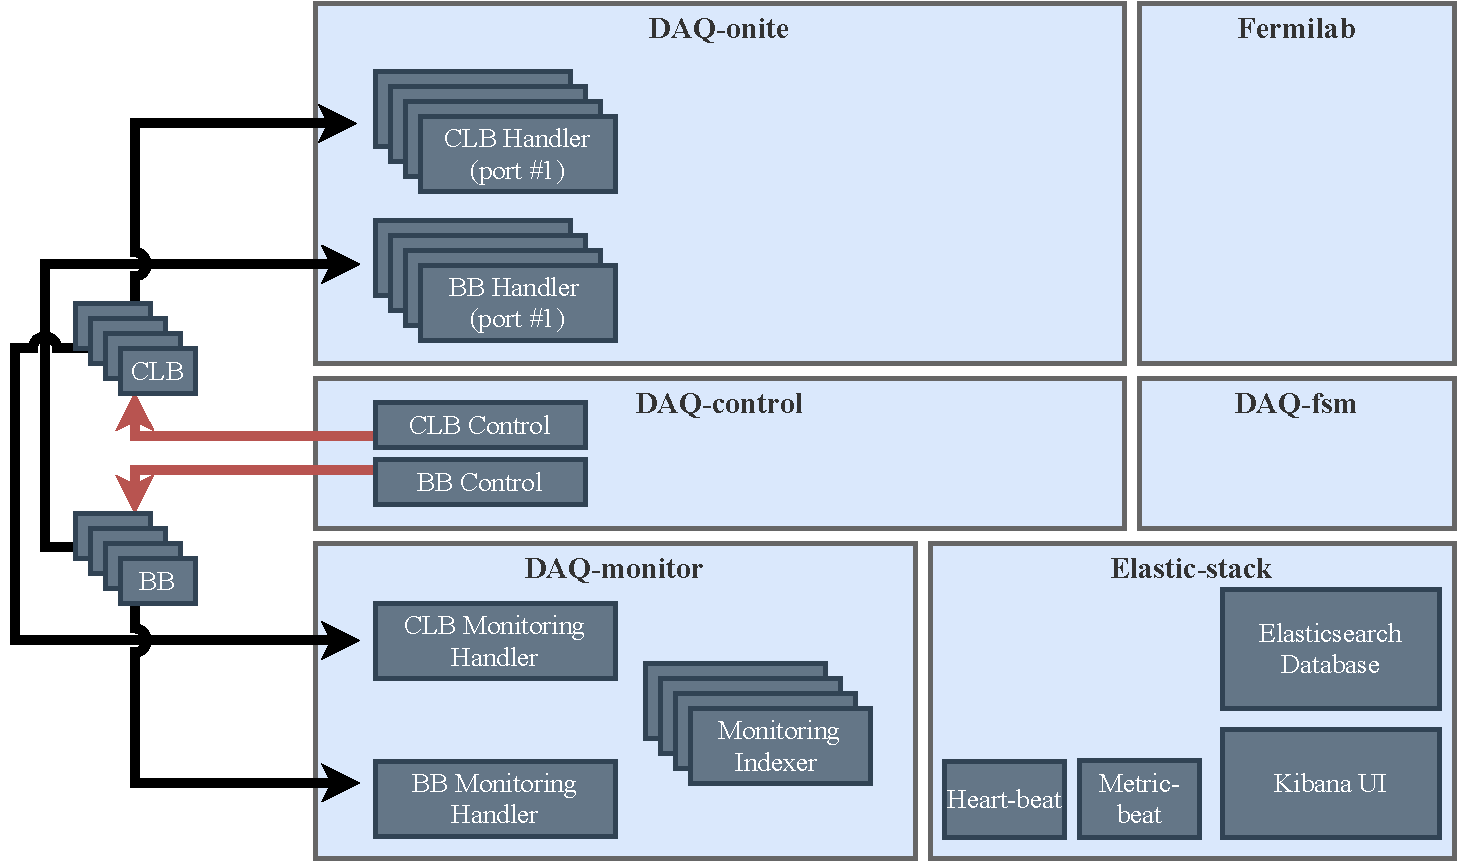
\includegraphics[width=\textwidth]{diagrams/5-daq/daq_software.pdf}
    \caption[Diagram of the \chipsfive software system in terms of the flow of data between
    components] {Diagram of the \chipsfive software system in terms of the flow of data between
    high-level components.}
    \label{fig:daq_software}
\end{figure}

The software itself is mainly written in C++ and can be found in the repository at
Ref.~\cite{chipsdaq2020}. The complete system is comprised of multiple processes, each of which is
illustratively shown within Fig.~\ref{fig:daq_software}, expressed in terms of the flow of data
between distinct software components. All DAQ processes make extensive use of multithreading and
asynchronous communication, principally implemented using the low-level Boost Asio (asynchronous
input/output) library~\cite{boost2020}. 

All central processing takes place on one of three machines: Shore DAQ-1 for hit handling, Shore
DAQ-2 control and monitoring, and Fermi DAQ-1 for \numi spill forwarding and storage. As the
processing of PMT hits is the principle software task, handled takes place exclusively on Shore
DAQ-1 without other processes to ensure maximum available processing power. Both Shore DAQ
machines have a backup machine (Shore DAQ-3 and Shore DAQ-4) to take over their functions in case
of a fault.

\subsection{Detector control} %%%%%%%%%%%%%%%%%%%%%%%%%%%%%%%%%%%%%%%%%%%%%%%%%%%%%%%%%%%%%%%%%%%%
\label{sec:daq_soft_control} %%%%%%%%%%%%%%%%%%%%%%%%%%%%%%%%%%%%%%%%%%%%%%%%%%%%%%%%%%%%%%%%%%%%%

All DAQ processes are controlled by a singular Finite State Machine (FSM) process. The FSM can be
in exactly one 

\begin{figure} % SOFTWARE DIAGRAM %
    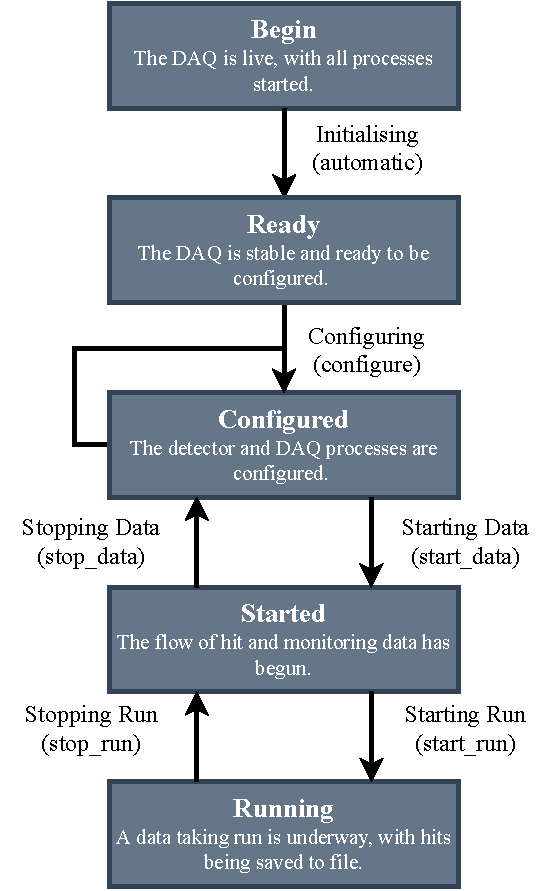
\includegraphics[width=0.6\textwidth]{diagrams/5-daq/fsm.pdf}
    \caption[fsm]
    {fsm}
    \label{fig:fsm}
\end{figure}

- inspired by the KM3NeT Java implementation
A singular Finite State Machine (FSM) process on DAQ
- Finite State Machine (FSM)
- DHCP server controls all the static ip addresses!
- Sometimes referred to as slow-control
- typically this is separated physically into a separate network, that is the best way to do the
DAQ for multiple reasons, but this would make the \chips DAQ system dramatically more complicated,
as running another cable requires so much more effort than normal, so they are combined into one.
- The detector is configured using a single human readable configuration file that defines all the
\textsc{Pom} types, MAC addresses, IP addresses, types, relay channels, which channels should be active and
their associate high voltage setting, threshold and electronic ID.
- Taking inspiration from the KM3NeT DAQ Java software
- Currently no run control system is in place to automatically control the detector according to a
scheduled run plan. Detector control is done via a simple command line interface (CLI) that
communicates with the FSM. Starting data taking, starting runs of a given type, stopping,
configuring with a given configuration file etc...

\subsection{Hit acquisition} %%%%%%%%%%%%%%%%%%%%%%%%%%%%%%%%%%%%%%%%%%%%%%%%%%%%%%%%%%%%%%%%%%%%%
\label{sec:daq_soft_hits} %%%%%%%%%%%%%%%%%%%%%%%%%%%%%%%%%%%%%%%%%%%%%%%%%%%%%%%%%%%%%%%%%%%%%%%%

As in done within KM3NeT, an `all-data-to-shore' approach is taken, where all PMT hit data is sent
via the WR network to the machines on shore. No triggering takes place within the detector. This
is done by collecting all PMT hits on each low level device (CLB or Beaglebone) within time
windows, \unit{10}{\mathrm{ms}} in length. At the end of each window, data is packaged along with
a header into User Datagram Protocol (UDP) packets and sent to shore. 

UDPavoids the overhead of error checking and correction processes, as this should be low it is not
required as allows for a higher bandwidth data stream to shore.

- How the beam spill stuffy works and how it is used to trigger hit acquisition
- Talk about the data rates for hits at full steam
- Jumbo frames etc
- Data is sent in UDP packets (not TCP so some will go missing)
- Typical ethernet frame has a maximum transmission unit (MTU) size of 1500 bytes, we use Jumbo
frames that allow for an MTU of 9000 bytes, this means we have a lot less small frames with only a
limited number of recorded hits, which proved to be taxing to the switches and lead to an increase
in the number of dropped frames.
- 1Gb links between WR switches, 10Gb link between FS switch and main DAQ machine. Provides
sufficient bandwidth, DO A SMALL CALCULATION!

\subsection{Monitoring} %%%%%%%%%%%%%%%%%%%%%%%%%%%%%%%%%%%%%%%%%%%%%%%%%%%%%%%%%%%%%%%%%%%%%%%%%%
\label{sec:daq_soft_monitor} %%%%%%%%%%%%%%%%%%%%%%%%%%%%%%%%%%%%%%%%%%%%%%%%%%%%%%%%%%%%%%%%%%%%%

- Talk about the data rates for monitoring at full steam
- Which machines run this, which is backup?

- Elasticsearch ref in~\cite{elastic2020}
- An open source RESTful, JSON-based, search engine and noSQL database.
- Data is stored in \emph{indices} in individual \emph{documents}
- Get to leverage an enormous amount of online support and the community
- daqlog: Uses for DAQ application logging with a severity
- daqstate: Used to report the current state of various DAQ applications
- monpom: Used for reporting general \textsc{Pom} monitoring information, such as temp, humidity, status
- monchannel: Used for reporting individual channel monitoring, such as rate, veto
- A series of altering rules are also set up constantly monitoring the status of the monitoring
data contained within the elasticsearch database to alert via slack or email individuals if something goes wrong.
- We index asynchronously to not block data taking, all data is backed up easily.
- Use the Kibana user interface which is accessible through a browser, means that no special
equipment, or GUIs are used, anyone on any machine has access to the full monitoring stack from
their browser. A series of dashboards ar set up to monitor everything within the detector.
- A series of indices are set up to store data which is sent via standard REST messages to the
database, the special indexing allows for quick `searching' over any time period etc... for
monitoring.
- Also means that anyone can quickly/easily look at any part of the data and make plots etc...
without needing to write an additional part of a monitoring program.
- Means the full detector and data quality monitoring is accessible to anyone with access anywhere
in the world via their normal browser.

\begin{figure} % MONITORING DIAGRAM %
    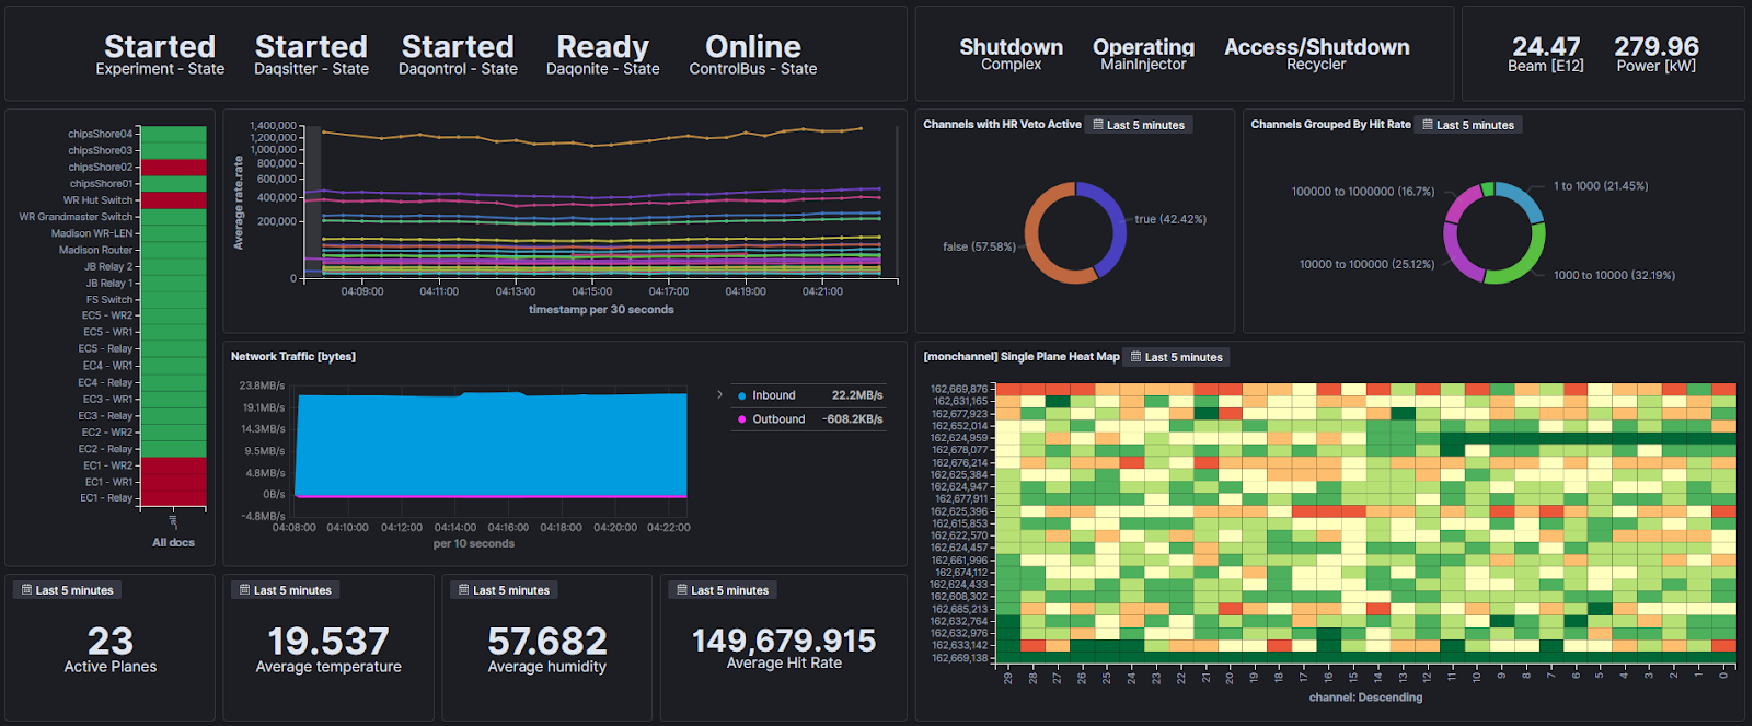
\includegraphics[width=\textwidth]{diagrams/5-daq/monitoring.pdf}
    \caption[monitoring short]
    {monitoring long}
    \label{fig:monitoring}
\end{figure}